\clearpage
\onecolumn
\section*{Appendix}
This section includes additional sample snapshots of malicious videos.
% \begin{figure}[htp]
%     \centering
%     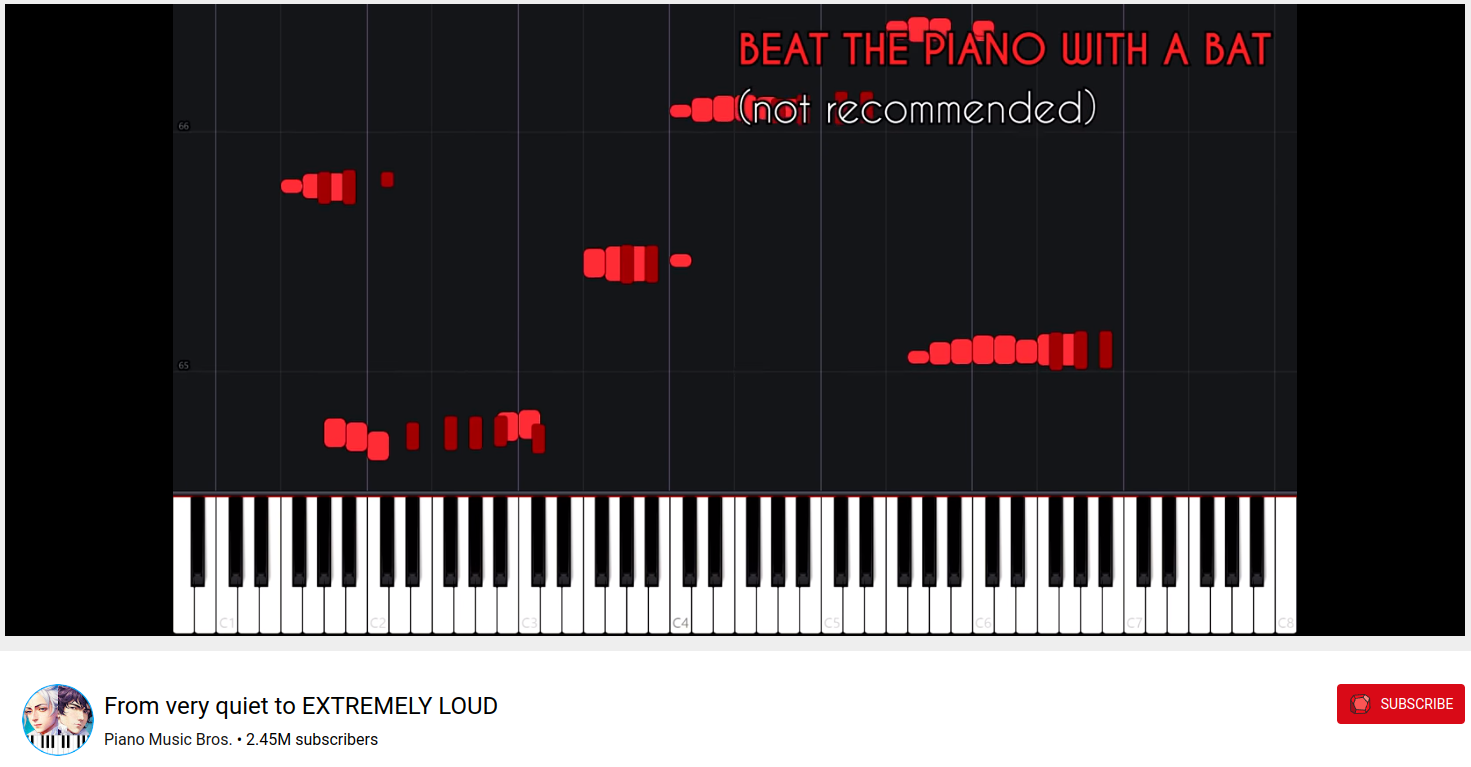
\includegraphics[width=0.6\columnwidth]{figures/malicious_audio.png}
%     \caption{A sample video which includes fast and loud piano notes. Usually in such videos, there is high tempo, no rhythm and varying pitches. The video also includes bright and striking hues, and also suggests a violent action of "hitting the piano with a bat"!}
%     \label{fig:ytkpiano}
% \end{figure}




\begin{figure}[!htb]
  \centering

  \begin{subfigure}{0.45\textwidth}
    \centering
    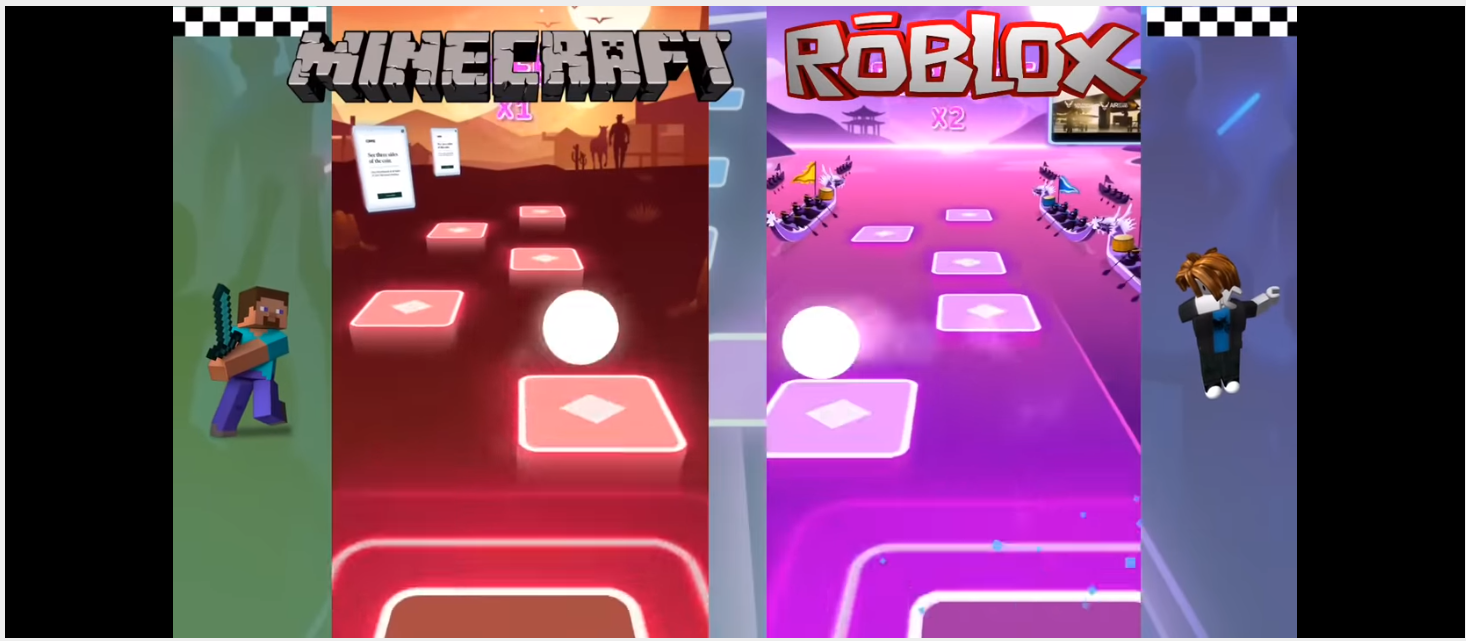
\includegraphics[width=\textwidth]{figures/malicious7.png}
    \caption{}
    \label{fig:image_a}
  \end{subfigure}
  \hfill
  \begin{subfigure}{0.45\textwidth}
    \centering
    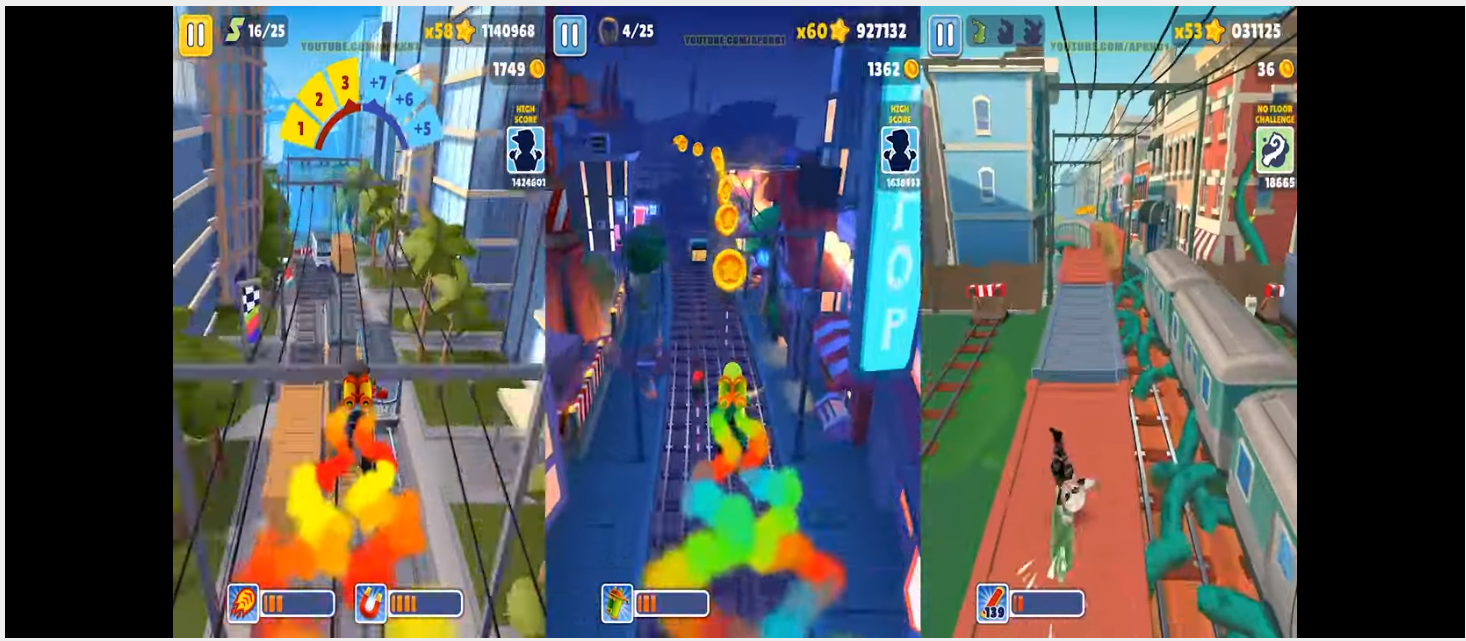
\includegraphics[width=\textwidth]{figures/malicious8.png}
    \caption{}
    \label{fig:image_b}
  \end{subfigure}

  \caption{a) shows a gameplay having striking colors which includes 2 different animations in 2 halves of the screen. b) shows a sample gameplay video for the Subway Surfer game displayed in a split-screen layout.}
  \label{fig:group_of_images}
\end{figure}

\begin{figure}[!htb]
  \centering

  \begin{subfigure}{0.45\textwidth}
    \centering
    
\includegraphics[width=0.8\textwidth]{figures/malicious5.png}
    \caption{}
    \label{fig:image_disgust}
  \end{subfigure}
  \hfill
  \begin{subfigure}{0.45\textwidth}
    \centering
    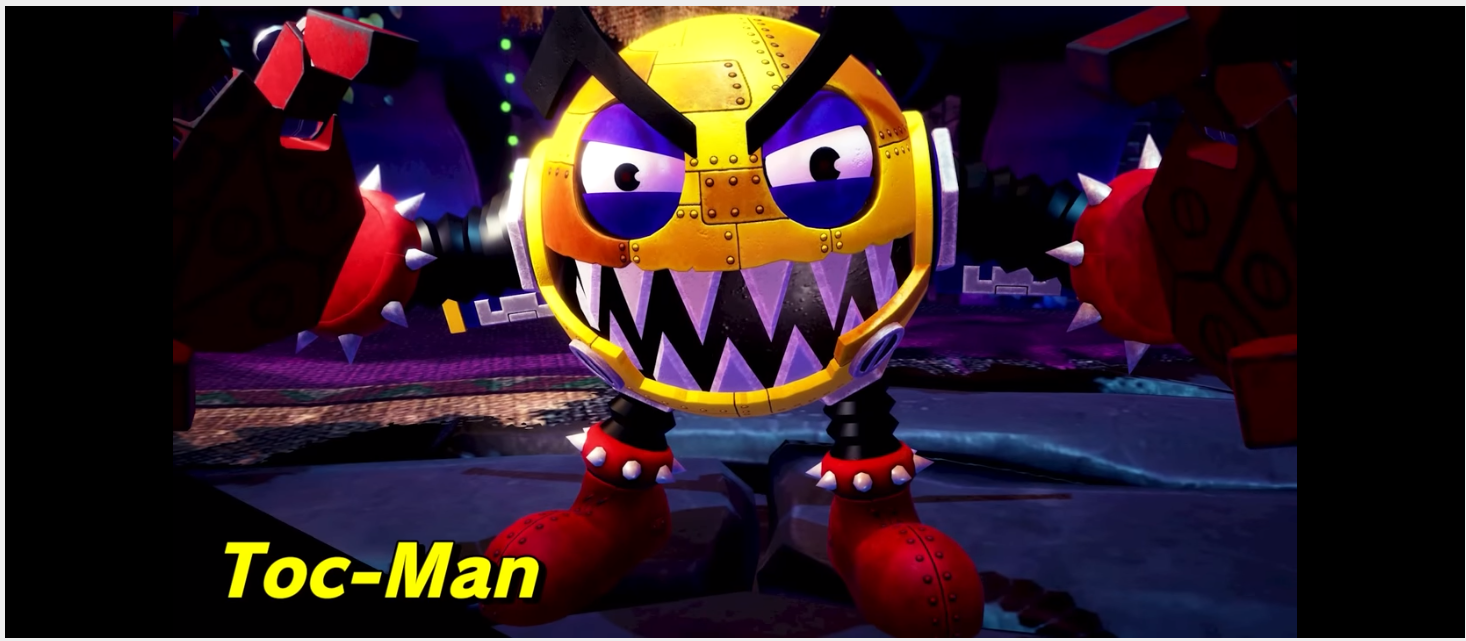
\includegraphics[width=\textwidth]{figures/malicious9.png}
    \caption{}
    \label{fig:image_angry}
  \end{subfigure}

  \caption{a) shows a disgusting and scary character b) shows a furious and frightening PacMan.}
  \label{fig:disgusting}
\end{figure}

\begin{figure*}[!h]
    \centering
    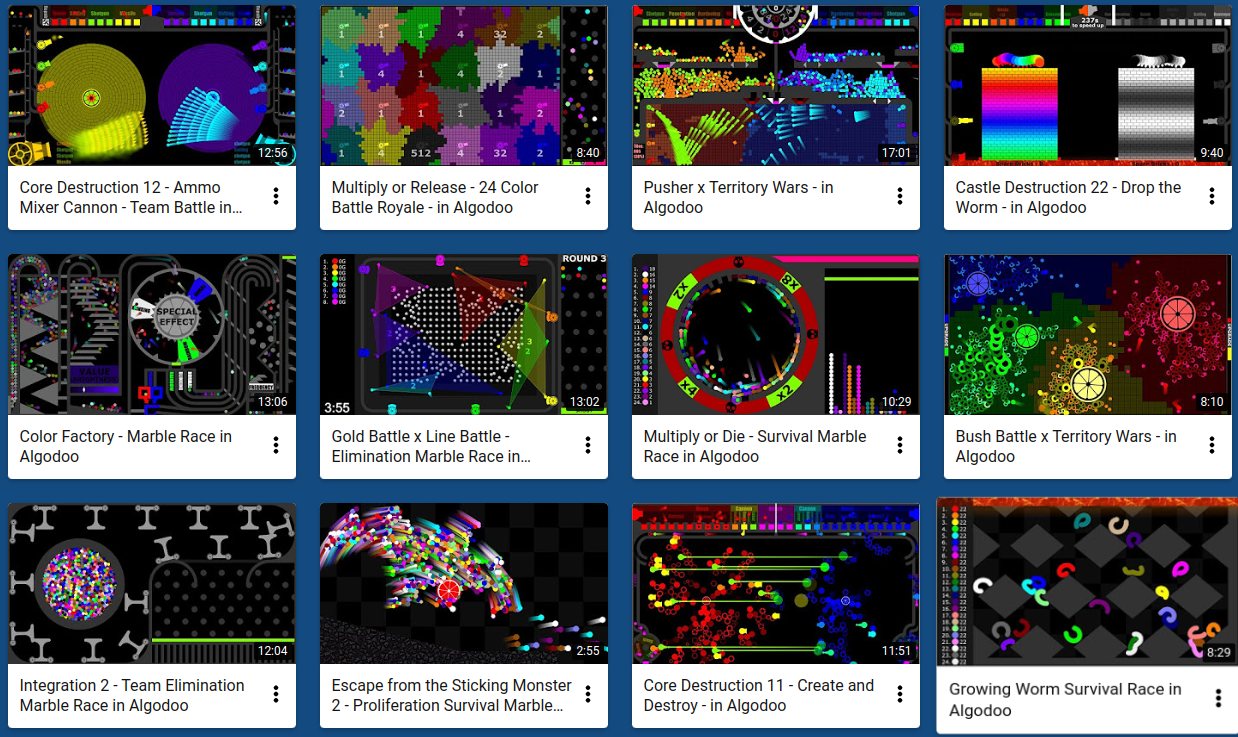
\includegraphics[width=0.8\textwidth]{figures/maliciou3.png}
    \caption{Videos of animations on YouTube Kids which include tiny fast-moving objects with bright colors.  The music soundtrack includes heavy metal and rock music.}  
    \label{fig:model}
\end{figure*}


% \begingroup
% \renewcommand{\arraystretch}{1.6}
% \begin{table}[h]
% \centering
% \begin{tabularx}{0.45\textwidth} { 
%   >{\raggedright\arraybackslash}X 
%   | >{\centering\arraybackslash}X 
%   | >{\centering\arraybackslash}X 
%   | >{\centering\arraybackslash}X
%   | >{\centering\arraybackslash}X 
%   | >{\centering\arraybackslash}X}
 
%  \textbf{Model} & \textbf{Layers} & \textbf{Patch Size} & \textbf{MLP Dim} & \textbf{Heads} & \textbf{Param} \\
%  \hline
%  \hline
%  ViT-B/16 & 12 & 16 & 3072 & 12 & 86M\\
%  ViT-B/32 & 12 & 32 & 3072 & 12 & 86M\\
%  % ViT-L/14 & 24 & 1024 & 4096 & 16 & 307M\\
% \end{tabularx}
% \caption{Comparison of CLIP base models.}
% \label{table:modelcomp}
% \end{table}
% \endgroup